\documentclass[10pt,letterpaper]{article}
\usepackage{multirow}
\usepackage{cogsci}
\usepackage{pslatex}
\usepackage{amsmath}
\usepackage{amsfonts}
\usepackage{setspace}
\usepackage{apacite}
\usepackage{graphicx}
\usepackage{caption}
\usepackage{subcaption}
\usepackage{etex}
\usepackage{color}
\usepackage[usenames,dvipsnames,svgnames,table]{xcolor}
\usepackage[usenames,dvipsnames]{xcolor}
\usepackage{tikz}
\usepackage{array}




%\usepackage{todonotes}

\usetikzlibrary{decorations.shapes}
\title{The Funny Thing About Incongruity: A Noisy Channel Model of Puns}
 
 \author{{\large {\bf Justine Kao$^1$} (justinek@stanford.edu)}, {\large {\bf Roger Levy$^2$} (rlevy@ucsd.edu)}, {\large {\bf Noah D.~Goodman$^1$} (ngoodman@stanford.edu)}\\
  $^1$Department of Psychology, Stanford University. $^2$Department of Linguistics, UCSD. }
 
 
%\author{{\large \bf Justine Kao (justinek@stanford.edu)} \\
%  Department of Psychology \\
%  Stanford, USA
%  \AND {\large \bf Noah Goodman (ngoodman@stanford.edu)} \\
%  Department of Psychology \\
%  Stanford, USA
%   \AND {\large \bf Roger Levy (rlevy@ucsd.edu)} \\
%  Department of Linguistics \\
%  UCSD, USA
%  }


\begin{document}

\maketitle

\begin{abstract}

``Researchers showed the robot ten puns, hoping that one of them would make it laugh. Unfortunately, no pun in ten did."

\textbf{Keywords:} 
Humor; language understanding; noisy channel; probabilistic models; sentence processing
\end{abstract}
\section{Introduction}
Humor plays an essential role in human interactions: it has important positive effects on children's development \cite{frank1989humor}, success in the work place \cite{duncan1990humor}, coping with illness and traumatic events \cite{johnson2002use, gelkopf1996humor}, and marital satisfaction \cite{ziv1989humor}.
Indeed, in a study on gender differences in desired characteristics of relationship partners, both men and women rated sense of humor as more important than physical attractiveness and earning potential \cite{stewart2000sex}. 
In this paper, we are interested in understanding how this fundamental and ubiquitous phenomenon works from the perspective of cognitive science. What makes something funny? How might the defining characteristics of humor shed light on the ways in which the mind processes and evaluates information?

A leading theory of humor posits that incongruity---perceiving a situation from different viewpoints and finding the resulting interpretations to be incompatible---contributes to sensations of mirth \cite{veale2004incongruity, forabosco1992cognitive, mcghee1979humor, martin2007psychology, hurley2011inside}; an idea that dates to Kant's theories about laughter and the sublime \cite{veatch1998theory, forabosco1992cognitive}. Although there is disagreement about whether incongruity alone is sufficient, most theorists accept that incongruity is necessary for producing humor: as Veale (2004) states, ``Of the few sweeping generalizations one can make about humor that are neither controversial or trivially false, one is surely that humor is a phenomenon that relies on incongruity." 
%(dating to Kant's theories about laughter and the sublime \cite{veatch1998theory, forabosco1992cognitive})
However, definitions of incongruity are often ambiguous and difficult to operationalize in empirical research. In this paper, we use a computational model of language understanding to formalize a notion of incongruity and tests its relationship to humor. 

Language understanding in general, and particularly humor, relies on rich commonsense knowledge, reasoning, and discourse understanding. To somewhat limit the scope of our task, we focus on applying formalizations of incongruity to a subset of linguistic humor: puns.
Writer and philosopher Henri Bergson defined a pun as ``a sentence or utterance in which two ideas are expressed, and we are confronted with only one series of words." This definition highlights the fact that one sentence must evoke two different interpretations in order to be a pun, which aligns with the concept of incongruity as a requisite of humor. 

We develop our model on homophone puns---puns that contain homophone words---because the space of possible interpretations of a homophone pun is relatively constrained and well-defined. An example helps to illustrate: 
\begin{itemize}
\item [] \emph{``The magician got so mad he pulled his hare out."} 
\end{itemize}
This sentence allows for two interpretations:
\begin{itemize}
\item[(a)] The magician got so mad he performed the trick of pulling a rabbit out of his hat.
\item[(b)] The magician got so mad he (idiomatically) pulled out the hair on his head.
\end{itemize}
If the comprehender interprets the word ``hare" as itself, he will arrive at interpretation (a); if he interprets the word as its homophone ``hair," he will arrive at interpretation (b). In other words, the sentence-level differences between interpretations (a) and (b) can be approximated by the two interpretations of the observed word ``hare." In general, distinct interpretations of a homophone pun hinges on one phonetically ambiguous word, allowing the two lexical forms of the homophone word to stand in for competing interpretations of the entire sentence. 

Critically, even though the example we gave was a written pun and the reader sees the word ``hare" explicitly on the page, the ``hair" interpretation is still present and even salient in the context of the sentence. 
%We propose that the reason why two ideas can be communicated through one set of words is because comprehenders maintain uncertainty about the input and consider alternative meanings distinct from what is directly observed. 
Noisy channel models of sentence processing posit that language comprehension is a rational process that incorporates uncertainty about the input at the word level to arrive at sentence-level interpretations that are globally coherent \cite{levy2008noisy, levy2009eye}. This process allows the comprehender to consider multiple word-level interpretations (``viewpoints'') to arrive at more than one interpretation of a sentence, each coherent but potentially incongruous with each other. The notion of incongruity thus fits naturally into a noisy channel model of sentence comprehension.

Our purposes for developing a formal model of linguistic humor are two-fold. First, we wish to formalize the concept of incongruity and test assumptions adopted by leading theories in humor research. Secondly, we aim to show that a noisy channel of language processing allows for flexible context selection and sentence comprehension that gives rise to sophisticated linguistic and social meaning such as humor. 

\section{Model}
Our model adopts a noisy channel approach in which a comprehender maintains uncertainty about an observed word and considers alternative interpretations. Given two candidate interpretations of the word, the comprehender determines whether one or both interpretations are likely by selectively using contextual information from the sentence. 

Previous research suggests that semantic priming plays an important role in lexical disambiguation during sentence processing. In particular, efficient processing of sentences that contain lexical ambiguity involves leveraging semantic association with neighboring words \cite{seidenberg1982automatic, simpson1981meaning, burke1984semantic}. Based on these findings, we propose that comprehenders use semantic information from the surrounding words to compute the probabilities of a candidate interpretation. Motivated by the incongruity theory of humor, we then predict that a sentence in which the target homophone word has two candidate interpretations that are similarly likely and supported by different viewpoints of the sentence is more likely to be funny. 

Suppose a sentence is composed of a vector of content words $\vec w = \{w_1, \dots ,w_n\}$ and a phonetically ambiguous word $h$ (remains to be decided if we want to say that $h$ is part of $\vec w$ or distinct). Since we assume that the candidate interpretations of $h$ are constrained by phonetic similarity, we make the simplifying assumption that only the two homophone interpretations of $h$ are salient and probable: $m_1$ and $m_2$. For example, in the magician pun described above, $h$ is the observed lexical item ``hare," and $m_1$ and $m_2$ are the interpretations \emph{hare} and \emph{hair}.

We propose a generative model of a sentence in which the latent variable $m$ and a latent indicator variable $\vec f$ are responsible for generating the observed words. $\vec f$ is a vector of indicator values that determines whether each word in a sentence is in semantic focus. When $f_i = 1$, $w_i$ is in semantic focus and is generated due to semantic relevance to $m$. Otherwise if $f_i = 0$, $w_i$ is simply drawn from a default unigram distribution. Similar approaches have been used in generative models of language to account for words that serve purposes in a sentence beyond providing semantic information, such as topic models that incorporate syntax \cite{griffiths2005integrating}. For our purposes, the indicator variable allows the model to consider subsets of the sentence as viewpoints that differentially support the two candidate interpretations of $h$. 
\begin{center}
\tikzset{decorate sep/.style 2 args=
{decorate,decoration={shape backgrounds,shape=circle,shape size=#1,shape sep=#2}}}
\begin{tikzpicture}
\tikzstyle{place}=[circle,draw,inner sep=2pt,minimum size=0.95cm]
 \tikzstyle{plate}=[rectangle,draw,inner sep=0pt]
 \node[place] (m) at (0,3) {$m$};
 \node[place] (w1) at (-2,1) {$w_1$};
 \node[place] (w2) at (-1,1) {$w_2$};
 \node[place] (h) at (0.5,1) {$h$}; 
 \node[place] (wn) at (2,1) {$w_n$};
 \node[place] (f1) at (-2, -0.5) {$f_1$};
 \node[place] (f2) at (-1, -0.5) {$f_2$};
\node[place] (fh) at (0.5, -0.5) {$f_h$};
\node[place] (fn) at (2, -0.5) {$f_n$};
 %\node[place] (wordsprior) at (0,4.5) {$\wordsprior$};
\draw [->] (m) -- (w1);
\draw [->] (m) -- (w2);
\draw [->] (m) -- (h);
\draw [->] (m) -- (wn);
\draw [->] (f1) -- (w1);
\draw [->] (f2) -- (w2);
\draw [->] (fh) -- (h);
\draw [->] (fn) -- (wn);
\draw[decorate sep={0.3mm}{1.65mm},fill] (-0.41,1) -- (-0.05,1);
\draw[decorate sep={0.3mm}{1.65mm},fill] (-0.41,-0.5) -- (-0.05,-0.5);
\draw[decorate sep={0.3mm}{1.65mm},fill] (1.09,1) -- (1.45,1);
\draw[decorate sep={0.3mm}{1.65mm},fill] (1.09,-0.5) -- (1.45,-0.5);
\end{tikzpicture}


\end{center}

Given our generative model and the observed words $w$ and $h$, we can infer the joint probability distribution of the latent variables $m$ and $\vec f$ given the observed words. This distribution can be factorized into:
$$
P(m, \vec f | \vec w) = P(m | \vec w) P(\vec f | m, \vec w) 
$$

We derive two measures separately from the factors $P(m | \vec w)$ and $P(\vec f | m, \vec w)$, which we will call ambiguity and disjointedness. Together, these two measures represent our formalization of incongruity. A sentence should support two interpretations (and is therefore ambiguous) in order to generate incongruous interpretations. In addition, the two interpretations should also be supported by different viewpoints of the sentence, which we approximate as the disjointedness of the subsets of the sentence that are in semantic focus with the two values of $m$. We derive these two measures more formally in the following paragraphs.

\subsubsection{Ambiguity} Let $M$ denote the distribution $P(m | \vec w)$, a binomial distribution over the two meaning values $m_1$ and $m_2$ given the observed words. If the entropy of this distribution $H(M)$ is low, this means that the probability mass is concentrated on only one meaning, and the alternative meaning is unlikely given the observed words. If $H(M)$ is high, on the other hand, this means that the probability mass is more evenly distributed among $m_1$ and $m_1$, and the two interpretations are similarly likely given the contexts. $H(M)$ is thus a natural measure of the degree of ambiguity present in a sentence. 

From conditional probability, we compute $P(m | \vec w)$ as follows:
$$
P(m | \vec w) = \sum_{\vec f} P(m, \vec f | \vec w) 
$$
From Bayes' theorem, this is proportional to the following:
$$
\sum_{\vec f} P(\vec w | m, \vec f) P(m) P(\vec f)= \sum_{\vec f} P(m)P(\vec f)\prod_i P(w_i | m, f_i)
$$
From the generative model, 
\[
    P(w_i | m, f_i) = 
\begin{cases}
    P(w_i),& \text{if } f=0\\
    P(w_i | m), &\text{if } f=1\\
\end{cases}
\]
We then compute the entropy of $P(m | w)$ as a measure of ambiguity.

\subsubsection{Disjointedness} Let $F_1$ denote the distribution $P(f | m_1, \vec w)$ and $F_2$ denote the distribution $P(f | m_2, \vec w)$. $F_1$ and $F_2$ represent the distributions over semantic focus sets given the observed words and $m_1$ and $m_2$, respectively. We use a symmetrised Kullback�Leibler divergence score $D_{KL}(F_1 || F_2) + D_{KL}(F_2 || F_1)$ to measure the distance between the two distributions. This score approximates the disjointedness of the semantic focus sets given $m_1$ and $m_2$. A low KL score would indicate that $m_1$ and $m_2$ are likely to be in semantic focus with similar subsets of the sentence; a high KL score would indicate that $m_1$ and $m_2$ are likely to be in semantic focus with different subsets of the sentence.

From conditional probability,
$$ 
P(\vec f | m, \vec w) \propto P(\vec f, \vec w | m) = P(\vec w | m, \vec f) P(\vec f | m)
$$
From the generative model, since $\vec f$ and $m$ are independent, $P(\vec f | m) = P(\vec f)$. We then compute the symmetrised KL divergence for $F_1$ and $F_2$ as a measure of disjointedness.

We have described a generative model of sentences containing phonetically ambiguous words that incorporates the idea of semantic focus sets. We then used the model to derive two measures that formalize incongruity. By combining a noisy channel model of language processing and standard information theoretic measures, our model presents a formalization of incongruity to be tested on humans' judgments of potentially humorous sentences.  

\section{Evaluation}
We evaluate our model and measures on a set of $235$ sentences, consisting of $65$ puns, $40$ ``de-punned" control sentences that are matched with a subset of the puns with certain manipulations described below, and $130$ control non-pun sentences that match the puns in containing the same phonetically ambiguous words. We evaluate our model based on how well it predicts people's funniness ratings of these sentences.
\subsection{Materials}
We selected $40$ pun sentences from a large collection of puns on a website called �Pun of the Day,� which contains over one thousand puns. Puns were selected such that the ambiguous item is a single phonetically ambiguous word, and such that no two puns in the collection have the same ambiguous item. To obtain more homophone pun items, a research assistant generated an addition $25$ pun sentences based on a separate list of homophone words.

We constructed $40$ sentences to be minimally different from the pun sentences that we collected from ``Pun of the Day," which we will call de-punned sentences. A second research assistant who was blind to the hypothesis was asked to replace one word in each of the pun sentences (without changing the homophone word itself) so that the sentence is still grammatical but is no longer a pun. This resulted in sentences that were only one word different from the pun sentences. 

The $130$ non-pun sentences were chosen to match each pun sentence on its ambiguous word as well as the alternative homophone. The sentences were taken from an online version of Heinle's Newbury House Dictionary of American English (http://nhd.heinle.com/). We selected sample sentences included in the definition of the homophone word. This design ensured that puns and non-pun sentences contain the same phonetically ambiguous words.

Below are example sentences from each category.\\\\
\begin{tabular}{| l | l |}\hline
\textbf{Type} & \textbf{Example} \\\hline
Pun & The magician got so mad he pulled his hare out. \\
De-pun & The professor got so mad he pulled his hare out.\\
Non-pun& The hare ran rapidly across the field.\\
Non-pun& Some people have lots of hair on their heads.\\\hline
\end{tabular}\\\\
\subsection{Human ratings of semantic relatedness}

As described in the model section, in order to compute our measures, we need the prior probabilities of the interpretations $P(m)$, the prior probabilities of the words $P(w)$, and the conditional probabilities of each word in the sentence given an interpretation $P(w | m)$. We computed $P(w)$ and $P(m)$ directly from the Google unigram corpus. However, $P(w | m)$ is difficult to obtain through corpora (due to data sparsity) as well as through empirical measures of association strength. Given these constraints, we approximate $P(w | m)$ using empirical measures of the semantic relatedness between $w$ and $m$, denoted as $R(c, m)$. We use $R(c, m)$ as a proxy for point wise mutual information between $c$ and $m$, defined as follows:
$$
R(w, m)= {\log \frac{P(w, m)}{P(w)P(m)}} = \log \frac{P(w | m)}{P(w)} = \log P(w | m) - \log P(w)
$$
With the proper substitutions and transformations, 
$$
P(w | m) = e^{R(w, m)} P(w)
$$
To obtain $R(w, m)$ for each of the words $w$ in the stimuli sentences, we recruited $200$ subjects on Amazon's Mechanical Turk to rate distinct word pairs on their semantic relatedness. Function words were removed from the sentences, and the remaining words were paired with each of the interpretations of the homophone sequence (e.g., ``magician" and ``hare" is a legitimate word pair, as well as ``magician" and ``hair"). This resulted in $1460$ distinct word pairs. Each subject saw $146$ pairs of words in random order and were asked to rate how related each word pair is from $1$ to $10$. The average split-half correlation of the relatedness ratings was $0.916$. 

Figure 1 and 2 show the relatedness of content words in the sentence with the two homophone interpretations. We see that in the pun sentence, the word ``magician" is rated as significantly more related to ``hare" than it is to ``hair", while the word ``pulled" is rated as significantly more related to ``hair" than it is to ``hare." On the other hand, all words in the non-pun example are significantly more related to the word ``hare" than to ``hair."

Figure 3 shows the average relatedness ratings of words and the two homophone interpretations across the three types of sentences. In pun sentences, the average relatedness of words to the two homophone interpretations are roughly equivalent. In the non-pun sentences, the average relatedness of words to the observed homophone is significantly higher than to the alternative homophone. This analysis of human ratings of relatedness supports the intuition on which our model is based that funnier sentences are those in which different contexts support incongruous interpretations of the homophone.

\begin{figure}[t]
\scalebox{0.4}{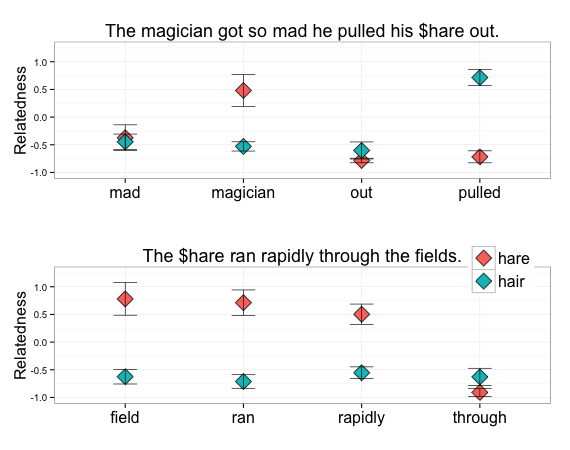
\includegraphics{Plots/relatedness_example.png}}
\caption{Relatedness of word pairs in example pun and non-pun.}
\end{figure}

\begin{figure}[t]
\scalebox{0.46}{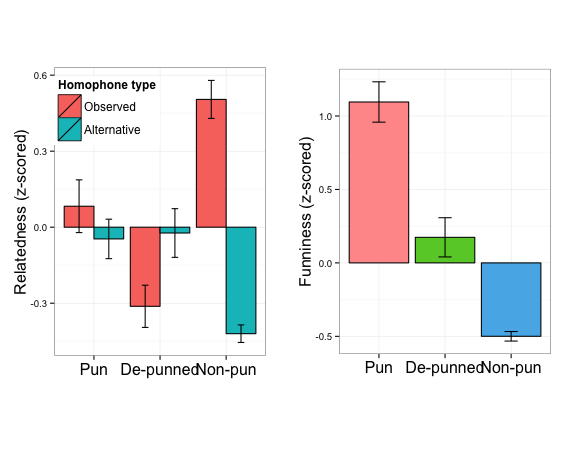
\includegraphics{Plots/ave_relatedness_funniness.png}}
\caption{Average relatedness and funniness ratings across sentence types}
\end{figure}


\subsection{Human Ratings of Funniness}
We obtained funniness ratings of the sentences from $100$ subjects on Amazon's Mechanical Turk. Each subject read $58$ - $59$ sentences in random order, counterbalanced for the sentence types, and rated each sentence on funniness and correctness. The average split-half correlation of the funniness ratings was $0.83$. Figure 4 shows the average funniness ratings of puns, non-puns, and de-punned sentences. Pun sentences are rated as significantly funnier than de-punned sentences, and de-punned sentences are rated as significantly funnier than non-pun sentences.


\section{Results}
We computed an ambiguity and disjointedness value for each of the $235$ sentences following the derivations described in the model section and using the relatedness measures described above. 

As predicted, ambiguity differs significantly across sentence types ($F(2, 232) = 11.94, p < 0.0001 $) and correlates significantly with human ratings of funniness across the $235$ sentences ($r = 0.27, p < 0.0001$). Furthermore, disjointedness differs significantly across sentence types as well ($F(2, 232) =  5.76, p < 0.005$) and correlates significantly with human ratings of funniness, although less strongly ($r = 0.21, p < 0.005$).


Using both ambiguity and disjointedness as the two dimensions that formalize incongruity, we can distinguish among puns, non-puns, and de-punned sentences. Both ambiguity and disjointedness measures are significant predictors of human ratings of funniness ($F(2,232) =19.6,  R^2 = 0.137, p < 0.001$).\\\\
\begin{tabular}{| l | r | r | l |}\hline
& {Estimate} & Std. Error & {p value} \\\hline
Intercept & $-0.687$ & $0.140$ & $1.75e^{-06}$ *** \\
Ambiguity & $1.011$ & $0.193$ & $3.49e^{-07}$ ***\\
Disjointedness & $0.237$ & $0.054$ & $1.81e^{-05}$ ***\\\hline
\end{tabular}\\\\


\begin{figure}[h]
\scalebox{0.45}{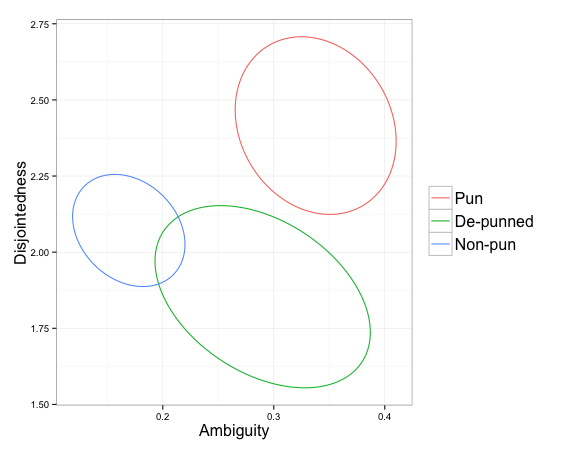
\includegraphics{Plots/ambiguity_disjointedness_ellipse.png}}
\caption{Standard error ellipses of ambiguity and disjointedness across sentence types}
\end{figure}


\begin{figure}[h]
\scalebox{0.47}{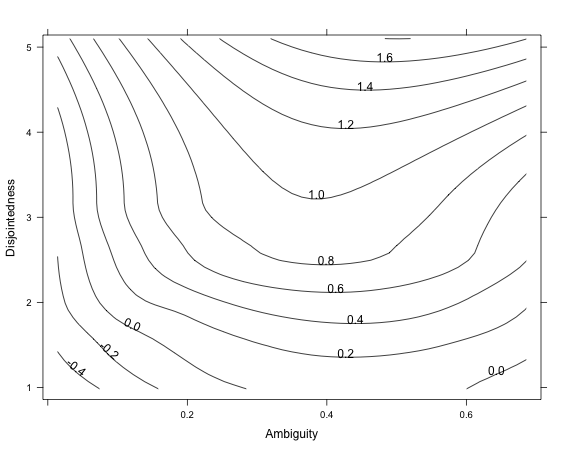
\includegraphics{Plots/contour_plot.png}}
\caption{Ambiguity and disjointedness with funniness contours}
\end{figure}

\subsubsection{Semantic focus sets}

Beyond predicting how funny a sentence is, our model can also tell us which particular features of a pun make it so amusing. By finding the semantic focus sets $\vec f$ that are most likely given the observed words and latent meaning variable $m$, we can identify words in a sentence that are likely to be in semantic focus given each of the two values of $m$. We present a few examples in the table below.
\begin{spacing}{2.5}
\begin{center}
\begin{table*}[ht]
\hfill{}
\begin{tabular}{|c|c|l|l|c|c|r|}
\hline
\textbf{$m1$}& \textbf{$m2$} & \textbf{Type} & \textbf{Semantic focus sets}& \textbf{Amb.} & \textbf{Disj.} & \textbf{Funniness}\\\hline
\multirow{4}{*}{{\color{Red} hare}} & \multirow{4}{*}{{\color{Emerald} hair}} & Pun & The \textbf{{\color{Red}magician}} got so mad he \textbf{{\color{Emerald}pulled}} his \textbf{{\color{Red}hare}} out. & $0.378$ & $2.291$ & $1.714$\\
&&De-pun & The professor got so mad he \textbf{{\color{Emerald} pulled}} his \textbf{{\color{Red} hare}} out. & $0.048$ & $1.832$ & $-0.103$\\
&&Non-pun & The \textbf{{\color{Red} hare}} \textbf{{\color{Red} ran}} \textbf{{\color{Red} rapidly}} through the \textbf{{\color{Red} fields}}. & $0.447$ &	$1.677$ &	$-0.400$\\
&&Non-pun & Most \textbf{{\color{Emerald} people}} have \textbf{{\color{Emerald} lots}} of \textbf{{\color{Emerald} hair}} on their \textbf{{\color{Emerald} heads}}. & $0.0004$ &	$2.807$ & $-0.343$ \\\hline
\multirow{4}{*}{{\color{Red} tiers}} & \multirow{4}{*}{{\color{Emerald} tears}} & Pun & It was an \textbf{{\color{Emerald} emotional}} \textbf{{\color{NavyBlue} wedding}}. Even the \textbf{{\color{Red} cake}} was in \textbf{{\color{Red} tiers.}} & $0.612$ & $2.311$ & $1.541$\\
&&De-pun & It was an \textbf{{\color{Emerald} emotional}} \textbf{{\color{NavyBlue} wedding}}. Even the \textbf{{\color{Emerald} mother-in-law}} was in \textbf{{\color{Red} tiers}}. & $0.189$ & $1.802$ &	$0.057$ \\

&&Non-pun & \textbf{{\color{Red} Boxes}} are \textbf{{\color{Red}stacked}} in \textbf{{\color{Red} tiers}} in the warehouse. & $0.194$ & 	$2.089$ &	$-0.560$\\

&&Non-pun & \textbf{{\color{Emerald} Tears}} ran down her \textbf{{\color{Emerald} cheeks}} as she watched a \textbf{{\color{Emerald} sad}} \textbf{{\color{Emerald} movie}}.& $0.0003$	& $3.283$ &	$-0.569$ \\
\hline
\end{tabular}
\hfill{}
\caption{Semantic focus sets of example sentences}
\label{tb:focusExamples}
\end{table*}
\end{center}
\end{spacing}


\section{Discussion}
\subsection{Mostly incomplete}
Given the prevalence of humor in human communication, researchers in artificial intelligence have argued that computers should be able to generate and detect humor in order to interact with humans more naturally and effectively \cite{mihalcea2006learning}. As a result, computational humor has made important progress and also received attention from popular press in the last decade (insert NYT citation here). However, most of the work in computational humor has focused either on utilizing joke-specific templates and schemata \cite{binsted1996machine, kiddon2011s}, or identifying linguistic features such as slang and alliteration that strongly predict humorous intent \cite{mihalcea2006learning, semantic2010}. The former type of studies is restricted to identifying jokes with a very specific format and structure, while the latter type falls short of testing or building upon deeper and more general theories of humor involving the management of incongruity. 

Our work moves beyond these two types of approaches and directly utilizes incongruence to identify humorous texts. Given that humor theorists view incongruity as an essential component of jokes, we examined whether human judgments of funniness can be predicted by the presence of incongruous interpretations of the same input. In particular, we developed a formal model of linguistic humor that fits naturally into the framework of normal language processing. We propose that a noisy channel approach to language processing allows the comprehender to consider alternative viewpoints and interpretations of the same linguistic input and can account for the possibility of incongruity. 

\subsubsection{Incomplete}
Describe its advantages over previous work on computational humor. Describe potential applications and generalizations to other forms of humor. 

\section{Acknowledgments}


\bibliographystyle{apacite}

\setlength{\bibleftmargin}{.125in}
\setlength{\bibindent}{-\bibleftmargin}

\bibliography{pun_bib}


\end{document}
